\date{}
\title{}
\date{}
\usepackage[outputdir=latex.out]{minted}
\begin{document}
\begin{frame}
    \titlepage
\end{frame}

\begin{frame}{last time}
    \begin{itemize}
    \item single-owner rule
    \item allowing borrowing
    \item tracking lifetime; annotations for lifetimes
    \item multiple readers, one writer
        \begin{itemize}
        \item avoiding inconsistencies re: pointers/etc. changing
        \end{itemize}
    \item rules conservative --- often prohibit ``actually safe'' things
    \end{itemize}
\end{frame}


\makeatletter
\newenvironment<>{btHighlight}[1][]
{\begin{onlyenv}#2\begingroup\tikzset{bt@Highlight@par/.style={#1}}\begin{lrbox}{\@tempboxa}}
{\end{lrbox}\bt@HL@box[bt@Highlight@par]{\@tempboxa}\endgroup\end{onlyenv}}

\newcommand<>\btHL[1][]{%
  \only#2{\begin{btHighlight}[#1]\bgroup\aftergroup\bt@HL@endenv}%
}
\def\bt@HL@endenv{%
  \end{btHighlight}%   
  \egroup %
}
\tikzset{
    btHLbox/.style={
        fill=red!30,outer sep=0pt,inner xsep=1pt, inner ysep=0pt, rounded corners=3pt
    },
}
\newcommand{\bt@HL@box}[2][]{%
  \tikz[#1]{%
    \pgfpathrectangle{\pgfpoint{1pt}{0pt}}{\pgfpoint{\wd #2}{\ht #2}}%
    \pgfusepath{use as bounding box}%
    \node[text width={},draw=none,anchor=base west, btHLbox, minimum height=\ht\strutbox+1pt,#1]{\raisebox{1pt}{\strut}\strut\usebox{#2}};
  }%
}

\lst@CCPutMacro
    \lst@ProcessOther {"2A}{%
      \lst@ttfamily 
         {\raisebox{2pt}{*}}% used with ttfamily
         {\raisebox{2pt}{*}}}% used with other fonts
    \@empty\z@\@empty

\lstdefinelanguage
   [x8664gas]{Assembler}     % add a "x64" dialect of Assembler
   [x86masm]{Assembler} % based on the "x86masm" dialect
   % with these extra keywords:
   {morekeywords={CDQE,CQO,CMPSQ,CMPXCHG16B,JRCXZ,LODSQ,MOVSXD,%
                  POPFQ,PUSHFQ,SCASQ,STOSQ,IRETQ,RDTSCP,SWAPGS,.TEXT,.STRING,.ASCIZ,%
                  BEQ,LW,SW,LB,SB,ADDIU,J,BEQZ,BNEZ,BNE,%
                  MOVUPD,MULPD,MOVSD,MULSD,%
                  SHLADD,MOV,CMP.LT,TBIT.NZ,BR.RET.SPTK.MANY,%
                  ADDQ,POPQ,PUSHQ,RRMOVQ,MRMOVQ,RMMOVQ,IRMOVQ,%
                  <-,LL,SC,ADDI,ADDL,VMOVDQA,ADDQ,CMPL,JB,JBE,MOVL,CLTQ,%
                  MOVW,PUSHW,MOV,ADD,SUB,INT,PUSH,MOV,ADD,REP,MOVSB,%
                  TESTQ,CMPQ,MOVL,MOVQ,ADDQ,JMPQ,XORQ,%
                  LEAQ,LEAL,LEA,RETQ,RET,POPL,POPW,PUSHL,PUSHW,%
                  LEAW,%
                  SUBQ,SYSCALL,.ASCII,CALLQ,MOVSLQ,JMP,ANDQ,SHRQ,MOVB,INCQ,TESTL,XORL,%
                  SHRL,LEAL,SARL,SUBL,IMULL,IMULQ,MOVDQU,PADDD,XORL,%
                  MOVZBL,MOVZB,SHRB,SRAL,SHRL,ANDL,%
                  CMOVNS,SRAL,SRAQ,MOVZBW,MOVZBQ,%
                  PADDW,PADDQ,MODUPS,MOVAPD,%
                  MOVL,RET,.GLOBL,%
		  PAUSE,LFENCE,JMP,%
                  },
    deletekeywords={eax,ebx,sp,si,cx,di,ds,cs,es,fs,dx,ax,bx,al,esi,ebp,ecx,rip,eip,edx,edi,rdi,esp},
    deletekeywords=[2]{size},
    alsoletter={\%},
    alsoother={()},
    emphstyle={\color{violet!50!black}},
    emph={\%rax,\%rbx,\%rcx,\%rdx,\%r8,\%r9,\%r10,\%r11,\%r12,\%r13,\%r14,\%r15,\%eax,\%ebx,\%sp,\%si,\%cx,\%di,\%ds,\%cs,\%es,\%fs,\%dx,\%ax,\%bx,\%al,\%esi,\%ebp,\%ecx,\%rip,\%eip,\%edx,\%edi,\%rdi,\%esp,\%rsp},
    %moreemph={eax,ebx,sp,si,cx,di,ds,cs,es,fs,dx,ax,bx,al,esi,ebp,ecx,rip,eip,edx,edi,rdi,esp},
    morecomment=[l]{\#},
    morecomment=[l]{\/\/},
    morecomment=[s]{/*}{*/},
    sensitive=false,
    keepspaces=true} % et

\lstalias[]{myasm}[x8664gas]{Assembler}

\lstdefinelanguage{JavaScript}{
  keywords={typeof, new, true, false, catch, function, return, null, catch, switch, var, if, in, while, do, else, case, break},
  ndkeywords={class, export, boolean, throw, implements, import, this},
  sensitive=false,
  comment=[l]{//},
  morecomment=[s]{/*}{*/},
  morestring=[b]',
  morestring=[b]"
}

\newcommand{\keywordstyle}{\sourcecodeprolight\bfseries\color{blue!30!black}}
\newcommand{\stringstyle}{\color{blue!20!black}\ttfamily}

\lstset{
    language=C,
    basicstyle=\sourcecodepro\EmptyMapping,
    escapechar=`,
    keywordstyle=\keywordstyle\EmptyMapping,
    identifierstyle=\sourcecodepro\EmptyMapping,
    numberstyle=\small\color{black!70},
    commentstyle=\color{red!60!black}\ttfamily\itshape,
    stringstyle=\color{blue!20!black}\ttfamily,
    ndkeywordstyle=\bfseries\color{blue!30!black},
    upquote=true,
}



\lstdefinestyle{medium}{
    basicstyle=\sourcecodepro\EmptyMapping\fontsize{12}{13}\selectfont,
    keywordstyle=\sourcecodepro\EmptyMapping\fontsize{12}{13}\selectfont\keywordstyle,
}

\lstdefinestyle{small}{
    basicstyle=\sourcecodepro\EmptyMapping\small,
    keywordstyle=\sourcecodepro\EmptyMapping\small\keywordstyle,
}

\lstdefinestyle{smaller}{
    basicstyle=\sourcecodepro\EmptyMapping\fontsize{11}{12}\selectfont,
    keywordstyle=\sourcecodepro\EmptyMapping\fontsize{11}{12}\selectfont\keywordstyle,
}

\lstdefinestyle{size105}{
    basicstyle=\sourcecodepro\EmptyMapping\fontsize{10.5}{11.5}\selectfont,
    keywordstyle=\sourcecodepro\EmptyMapping\fontsize{10.5}{11.5}\selectfont\keywordstyle,
}

\lstdefinestyle{size10}{
    basicstyle=\sourcecodepro\EmptyMapping\fontsize{10}{11}\selectfont,
    keywordstyle=\sourcecodepro\EmptyMapping\fontsize{10}{11}\selectfont\keywordstyle,
}

\lstdefinestyle{size9}{
    basicstyle=\sourcecodepro\EmptyMapping\fontsize{9}{10}\selectfont,
    keywordstyle=\sourcecodepro\EmptyMapping\fontsize{9}{10}\selectfont\keywordstyle,
}
\lstdefinestyle{size8}{
    basicstyle=\sourcecodepro\EmptyMapping\fontsize{8}{9}\selectfont,
    keywordstyle=\sourcecodepro\EmptyMapping\fontsize{8}{9}\selectfont\keywordstyle,
}



\lstdefinestyle{script}{
    basicstyle=\sourcecodepro\EmptyMapping\scriptsize,
    keywordstyle=\sourcecodepro\EmptyMapping\scriptsize\bfseries,
}




\begin{frame}{aside: anonymous feedback}
    \begin{itemize}
    \item ``Please teach us about web based exploitation.''
    \item area I'm not super familiar with
    \item major topics in this area seem covered in 3710
        \begin{itemize}
        \item XSS 
        \item CSRF (some versions of 3710; maybe not Orebaughs?)
        \end{itemize}
    \item some potential areas, but seem rather niche
        \begin{itemize}
        \item turning XSS into useful exploit (but not much to say?)
        \item security with embedded other pages/user content
        \item web tracking/privacy (is this the right class for that?)
        \item restricting browser extensions
        \end{itemize}
    \end{itemize}
\end{frame}

\section{destructors}
\begin{frame}[fragile]{Rust dropping (1)}
\begin{minted}[fontsize=\fontsize{9}{10}\selectfont]{Rust}
struct Example {}

impl Drop for Example {
    fn drop(&mut self) {
        println!("in Example's drop")
    }
}

fn main() {
    {
        let t = Example {};
        println!("A");
    }
    println!("B");
}
\end{minted}
output: A(newline)in Example's drop(newline)B
\end{frame}

\begin{frame}[fragile]{Rust dropping (2)}
\begin{minted}[fontsize=\fontsize{9}{10}\selectfont]{Rust}
struct Example {}

impl Drop for Example {
    fn drop(&mut self) {
        println!("in Example's drop")
    }
}

fn main() {
    let q: Example;
    {
        let t = Example {};
        println!("A");
        q = t;
    }
    println!("B");
}
\end{minted}
output: A(newline)B(newline)in Example's drop
\end{frame}

\begin{frame}[fragile]{Rust dropping (3)}
\begin{minted}[fontsize=\fontsize{9}{10}\selectfont]{Rust}
#[derive(Clone)] struct Example {}

impl Drop for Example {
    fn drop(&mut self) {
        println!("in drop")
    }
}

fn main() {
    let q: Example;
    {
        let t = Example {};
        println!("A");
        q = t.clone();
    }
    println!("B");
}
\end{minted}
output: A(newline)in drop(newline)B(newline)in drop
\end{frame}

\begin{frame}{preview: wrapper objects as tool}
    \begin{itemize}
    \item to manage memory, make objects with custom \texttt{drop} functions
    \item creating object: allocates memory; droping: frees memory
    \vspace{.5cm}
    \item Rust compiler will insert drop calls automatically
    \item \ldots and borrowing will enforce error if object still in use
    \end{itemize}
\end{frame}

\begin{frame}{aside: RAII and C++}
    \begin{itemize}
    \item common C++ idea that Rust is copying: \\
        \textit{Resource Acquisition is Initialization} (RAII)
    \item will show ``smart pointer'' types where idea prominent in C++
    \item \ldots but C++ lacks compiler borrowing/etc. enforcement
    \vspace{.5cm}
    \item idea probably didn't start with C++, though most prominent current version
    \end{itemize}
\end{frame}



\section{Rust: escape hatches and supporting dynamic allocation}
\begin{frame}{what about dynamic allocation?}
    \begin{itemize}
    \item saw Rust's Vec class --- equivalent to C++ vector/Java ArrayList
    \item idea: Vec wraps a heap allocation of an array
    \item owner of Vec ``owns'' heap allocation
        \begin{itemize}
        \item delete when no owner
        \end{itemize}
    \item also Box class --- wraps heap allocation of a single value
        \begin{itemize}
        \item basically same as Vec except one element
        \end{itemize}
    \end{itemize}
\end{frame}


\subsection{escape hatches implementing Vec}

\begin{frame}{escape hatch}
    \begin{itemize}
    \item Rust lets you avoid compiler's mechanisms
    \item implement your own
    \item \textbf{unsafe} keyword
    \item how Vec is implemented
    \end{itemize}
\end{frame}

\begin{frame}[fragile,label=insideVec]{deep inside Vec}
\begin{minted}[fontsize=\fontsize{9}{10}\selectfont]{Rust}
pub struct Vec<T> {
    buf: RawVec<T>, // interface to malloc
    len: usize,
}

impl<T> Vec<T> {
    ...
    pub fn truncate(&mut self, len: usize) {
        unsafe {
            // drop any extra elements
            while len < self.len {
                // decrement len before the drop_in_place(), so a panic on Drop
                // doesn't re-drop the just-failed value.
                self.len -= 1;
                let len = self.len;
                ptr::drop_in_place(self.get_unchecked_mut(len));
            }
        }
    }
    ...
}
\end{minted}
\end{frame}




\subsection{raw pointers}
\begin{frame}[fragile]{raw pointers (1)}
\begin{minted}[fontsize=\fontsize{12}{13}]{Rust}
fn main() {
    let mut y: Vec<u32> = vec![10,20,30,40];
    let x: *mut u32 = &mut y[0];
    println!("{:?}", x);
        // 0x5d82222f9b10
    println!("{}", unsafe{*x});
        // 10
    println!("{}", unsafe{*(x.wrapping_add(1))});
        // 20
    unsafe{*x = 11};
    println!("{:?}", y);
        // [11, 20, 30, 40]
}
\end{minted}
\end{frame}

\begin{frame}[fragile]{raw pointers (2)}
\begin{minted}[fontsize=\fontsize{12}{13}]{Rust}
fn main() {
    let z: &mut u32;
    {
        let mut y: Vec<u32> = vec![10,20,30,40];
        let x: *mut u32 = &mut y[0];
        z = unsafe {&mut *x};
        *z = 12;
        println!("{}", z);
            // 12
        println!("{:?}", y);
            // [12, 20, 30, 40]
    }
    println!("{}", z);
        // 1134576980 (accesses freed memory!)
}
\end{minted}
\end{frame}

\begin{frame}[fragile]{raw pointers (3)}
\begin{minted}[fontsize=\fontsize{12}{13}]{Rust}
use libc;

fn main() {
    let x: *mut u32 = unsafe { libc::malloc(16) as *mut u32 };
    let pointer_value: usize = x as usize;
    println!("{:?} {:#x}", x, pointer_value);
        // 0x58a7196d5b10 0x58a7196d5b10
    unsafe{*x = 0x123456;}
    unsafe{*(x.wrapping_add(1)) = 0x234567;}
    let y: *mut u32 = (pointer_value+1) as *mut u32;
    println!("{:#x}", unsafe{*y});
        // release mode: 0x67001234
        // debug mode: thread 'main' panicked at src/main.rs:10:30:
        //      misaligned pointer dereference: ....
}
\end{minted}
\end{frame}

\begin{frame}{unsafe action at a distance}
    \begin{itemize}
    \item raw pointers = like pointers in C, basically
    \item need \texttt{unsafe} keyword to use
    \item need to explicitly dereference (*) to read unlike references
    \vspace{.5cm}
    \item can be used to create normal references
    \item \ldots if done incorrectly, can cause all sorts of problems
    \end{itemize}
\end{frame}


% FIXME: RefCell

\subsection{implementing new sharing schemes}
\subsubsection{Rc}
\begin{frame}<1>[fragile,label=escapeHatchSupportRc]{Rust escape hatch support}
    \begin{itemize}
        \item escape hatch: make new reference-like object
            \begin{itemize}
            \item (\ldots implemented by returning temporary `real' references)
            \end{itemize}
        \item<2> Rc: \verb|Rc<T>| acts like \verb|&T|
        \item callbacks on ownership ending (normally deallocation)
            \begin{itemize}
            \item Rust compiler enforces that ref-like object not in use when free call made
            \end{itemize}
        \item<2> Rc: deallocating \verb|Rc<T>| decrements shared count
        \item<2> Rc: real object only decremented on count == 0
        \item choice of what happens on copy
        \item<2> Rc: no implicit copy; explicit \verb|clone| operation increments count
    \end{itemize}
\end{frame}
 
\begin{frame}[fragile,label=refCounting]{alternative rule: reference counting}
    \begin{itemize}
    \item keep track of number of references
    \item increment count when making new `clone' of reference
    \item decrement when reference goes away
        \begin{itemize}
        \item Rust borrowing rules will enforce it is not used when this happens
        \end{itemize}
    \item delete when count goes to zero
        \begin{itemize}
        \item Rust automatically calls destructor --- no programmer effort
        \end{itemize}
    \item explicit operation to make new reference
    \item Rust implement with Rc type (``counted reference'')
    \end{itemize}
\end{frame}

\begin{frame}[fragile,label=refCountingEx]{Ref Counting Example}
\begin{minted}[fontsize=\fontsize{9}{10}\selectfont]{Rust}
struct Grade {
    score: i32, studentName: String, assignmentName: String,
}
struct Student {
    name: String,
    grades: Vec<Rc<Grade>>,
}
struct Assignment {
    name: String,
    grades: Vec<Rc<Grade>>
}

fn add_grade(student: &mut Student, assignment: &mut Assignment, score: i32) {
    let grade = Rc::new(Grade {
        score: score,
        studentName: student.name.clone(),
        assignmentName: assignment.name.clone(),
    })
    student.grades.push(Rc::clone(&grade));
    assignment.grades.push(Rc::clone(&grade));
    println!("Added grade with score={}", grade.score);
}
\end{minted}
\end{frame}

\againframe<2>{escapeHatchSupportRc}

\begin{frame}[fragile,label=rcImplA]{Rc implementation (approx) (0)}
\begin{minted}[fontsize=\fontsize{10}{11}\selectfont]{Rust}
struct RcInner<T: ?Sized> {
    strong: Cell<usize>,    // <-- count of Rc<T>s pointing to this
    weak: Cell<usize>,      // <-- count of Weak<T>s pointing to this
    value: T,               // <-- actual data
}

pub struct Rc<T: ?Sized> {
    ptr: NonNull<RcInner<T>>,
    phantom: PhantomData<RcInner<T>>, // <- so compiler infers what operations are safe better
}
\end{minted}
\begin{itemize}
\item NonNull = raw pointer wrapper
\item Cell = way to have mutable field of immutable object
\end{itemize}
\end{frame}



\begin{frame}[fragile,label=rcImplA]{Rc implementation (approx) (1)}
\begin{minted}[fontsize=\fontsize{10}{11}\selectfont]{Rust}
impl<T: ?Sized> Clone for Rc<T> {
    ... 
    fn clone(&self) -> Rc<T> {
        self.inc_strong(); // <-- increment reference count
        Rc { ptr: self.ptr }
    }
}
\end{minted}
\end{frame}

\begin{frame}[fragile,label=rcImplB]{Rc implementation (approx) (2)}
\begin{minted}[fontsize=\fontsize{10}{11}\selectfont]{Rust}
unsafe impl<#[may_dangle] T: ?Sized> Drop for Rc<T> {
    ...
    fn drop(&mut self) { // <-- compilers calls on deallocation
        unsafe {
            self.inner().dec_strong();
            if self.inner().strong() == 0 {
                self.drop_slow();
            }
        }
    }
    ...
}
\end{minted}
\end{frame}

\begin{frame}[fragile,label=rcImplC]{Rc implementation (approx) (3)}
\begin{minted}[fontsize=\fontsize{10}{11}\selectfont]{Rust}
impl<T: ?Sized> Deref for Rc<T> {
    type Target = T;

    #[inline(always)]
    fn deref(&self) -> &T {
        &self.inner().value
    }
}
\end{minted}
\begin{itemize}
\item observation: returned reference still has lifetime
\item compiler will enforce that extracted reference only used when Rc object valid
\end{itemize}
\end{frame}


\begin{frame}{Rc limitations}
    \begin{itemize}
    \item Rc: only gives references to \textit{read-only} objects
        \begin{itemize}
        \item cannot enforce ``only one mutable reference'' rule
        \end{itemize}
    \item Rc: allows memory leaks via circular references
        \begin{itemize}
        \item correct way to handle ciruclar references: Weak
        \item \ldots but not enforcement that it is used when needed
        \end{itemize}
    \end{itemize}
\end{frame}

\begin{frame}[fragile]{aside: Weak}
\begin{minted}[fontsize=\fontsize{10}{11}\selectfont]{Rust}
struct Foo {
    my_bar: Rc<Bar>,
    ...
}
struct Bar {
    my_foo: Weak<Foo>.
    ...
}
...
let bar: Bar = ...;
...
match bar.my_foo.upgrade() {
    Some(foo_rc) => {
        // foo_rc is an Rc<Foo>
        ...
    },
    None => {
        // the foo object was deleted
    }
}
\end{minted}
\end{frame}



\subsection{non-Rust smart pointers}
\begin{frame}{C++ has `smart pointers'}
    \begin{itemize}
    \item probably what inspired Rust Box, Rc, etc.
    \vspace{.5cm}
    \item \texttt{std::shared\_ptr} (like Rc), \texttt{std::unique\_ptr} (like Box)
        \begin{itemize}
        \item like Rust Deref/DerefMut, implement \texttt{operator*} and \texttt{operator->} to act
            like `normal' pointers
        \end{itemize}
    \item like Rust, internally return temporary real references
    \vspace{.5cm}
    \item problem: no compiler enforcement of ownership rules
    \item can accidentally use real reference when it is invalid
    \end{itemize}
\end{frame}


\subsubsection{RefCell}
\begin{frame}<0>[fragile,label=escapeHatchSupportRefCell]{Rust escape hatch support}
    \begin{itemize}
        \item escape hatch: make new reference-like types
            \begin{itemize}
            \item (\ldots implemented by returning temporary `real' references)
            \end{itemize}
        \item<2> RefCell: \verb|borrow_mut()| method gives mutable-ref-like object
            \begin{itemize}
            \item crashed if conflicting borrowing active
            \end{itemize}
        \item<2> RefCell<T> \verb|x|: \verb|x.borrow()| gives immutable-ref-like object
            \begin{itemize}
            \item crashed if conflicting borrowing active
            \end{itemize}
        \item callbacks on ownership ending (normally deallocation)
            \begin{itemize}
            \item Rust compiler enforces that ref-like object not in use when free call made
            \end{itemize}
        \item<2> RefCell<T> --- deallocate normally
        \item choice of what happens on move/copy
        \item<2> RefCell<T> ---- no implicit copy; explicit clone makes clone of T
    \end{itemize}
\end{frame}

\begin{frame}[fragile]{alternate rule: tracked usage}
    \begin{itemize}
    \item runtime-enforced version of Rust borrowing rules
    \item \texttt{borrow\_mut()}: give \verb|&mut T|-like object only if other active borrows
        \begin{itemize}
        \item increment counter of active mutable borrows (instead of tracking statically)
        \item decrement counter when \verb|&mut T| no longer in use 
        \end{itemize}
    \item \texttt{borrow()}: give \verb|&T|-like object only if no active mutable borrows
        \begin{itemize}
        \item increment counter of active immutable borrows
        \item decrement counter when \verb|&T| no longer in use
        \end{itemize}
    \end{itemize}
\end{frame}

\begin{frame}[fragile]{RefCell example (0)}
\begin{minted}[fontsize=\fontsize{9}{10}]{Rust}
fn myadd(x: &RefCell<i32>, y: &RefCell<i32>, z: &RefCell<i32>) {
    let mut x_value = x.borrow_mut();
    let y_value = y.borrow();
    let z_value = z.borrow();
    *x_value += *y_value;
    *x_value += *z_value;
    println!("{}, {}, {}", x_value, y_value, z_value);
}

fn main() {
    let x: RefCell<i32> = RefCell::new(1);
    let y: RefCell<i32> = RefCell::new(2);
    let z: RefCell<i32> = RefCell::new(3);
    
    myadd(&x, &y, &z); // 6, 2, 3
    myadd(&x, &y, &y); // 10, 2, 2
    myadd(&x, &x, &x); // RUNTIME ERROR
}
\end{minted}
\end{frame}

\begin{frame}[fragile]{RefCell example (1)}
\begin{minted}[fontsize=\fontsize{9}{10}]{Rust}
fn appendsum(x: &RefCell<Vec<i32>>, y: &RefCell<Vec<i32>>, z: &RefCell<Vec<i32>>) {
    let mut x_value = x.borrow_mut();
    let y_value = y.borrow();
    let z_value = z.borrow();
    let i = 0;
    for (y_number, z_number) in y_value.iter().zip(z_value.iter()) {
        x_value.push(y_number + z_number);
    }
    println!("{:?}", *x_value)
}

fn main() {
    let x: RefCell<Vec<i32>> = RefCell::new(vec![1]);
    let y: RefCell<Vec<i32>> = RefCell::new(vec![2]);
    let z: RefCell<Vec<i32>> = RefCell::new(vec![3]);
    
    appendsum(&x, &y, &z);
    appendsum(&x, &y, &y);
    appendsum(&x, &x, &x);
}
\end{minted}
\end{frame}

\againframe<2>{escapeHatchSupportRefCell}

\begin{frame}[fragile]{approx RefCell implementation (1)}
\begin{minted}[fontsize=\fontsize{9}{10}]{Rust}
pub struct RefCell<T: ?Sized> {
    // mutable integer
        // set to -1 on mutable borrow
        // incremented on immutable borrow
    borrow: Cell<BorrowFlag>,
    value: UnsafeCell<T>,
}

pub fn borrow_mut(&self) -> RefMut<'_, T> { ... }

pub struct RefMut<'b, T: ?Sized + 'b> {
    value: NonNull<T>,
    borrow: BorrowRefMut<'b>,
    ...
}
\end{minted}
\begin{itemize}
\item RefMut = type that acts like reference (\texttt{Deref}, \texttt{DerefMut})
\item BorrowRefMut = contains pointer to Cell<BorrowFlag>, handles updates
\end{itemize}
\end{frame}

\begin{frame}[fragile]{approx RefCell implementation (RefMut)}
\begin{minted}[fontsize=\fontsize{9}{10}]{Rust}
pub struct RefMut<'b, T: ?Sized + 'b> {
    value: NonNull<T>,
    borrow: BorrowRefMut<'b>,
    ...
}

impl<T: ?Sized> DerefMut for RefMut<'_, T> {
    fn deref_mut(&mut self) -> &mut T {
        unsafe { self.value.as_mut() }
    }
}
\end{minted}
\end{frame}


\begin{frame}[fragile]{approx RefCell implementation (BorrowRefMut)}
\begin{minted}[fontsize=\fontsize{9}{10}]{Rust}
struct BorrowRefMut<'b> {
    borrow: &'b Cell<BorrowFlag>,
}
impl Drop for BorrowRefMut<'_> {
    fn drop(&mut self) {
        let borrow = self.borrow.get(); self.borrow.set(borrow + 1);
    }
}
impl<'b> BorrowRefMut<'b> {
    fn new(borrow: &'b Cell<BorrowFlag>) -> Option<BorrowRefMut<'b>> {
        match borrow.get() {
            UNUSED => {
                borrow.set(UNUSED - 1); Some(BorrowRefMut { borrow })
            }
            _ => None,
        }
    }
}
\end{minted}
\end{frame}



\subsection{assignment}
\begin{frame}{assignment}
    \begin{itemize}
    \item Rust program that uses unsafe/raw pointers
    \item has use of pointers that violates single-owner idea
    \vspace{.5cm}
    \item your task: change it to be all safe
    \end{itemize}
\end{frame}

\subsection{aside: concurrency + UAF}
\begin{frame}{example: concurreny UAF bug}
\begin{tikzpicture}
\node (fig) {
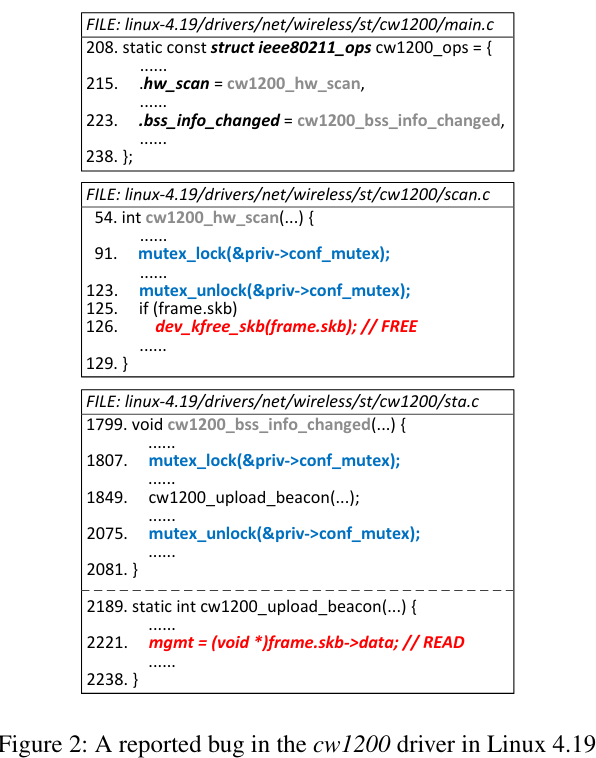
\includegraphics[height=0.9\textheight]{../betterpl/linux-conc-uaf-fig}
};
\node[anchor=north west,font=\small,align=left] at (fig.north east) {
Figure from Bai, Lawall, Chen and Mu \\ (Usenix ATC'19) \\
{\scriptsize ``Effective Static Analysis of Concurrency} \\ {\scriptsize Use-After-Free Bugs in Linux drivers''} \\
~ \\
bug in a wireless networking driver
};
\end{tikzpicture}
\end{frame}


\subsection{concurrency}
\begin{frame}{data races}
    \begin{itemize}
    \item Rusts rules around modification built assuming concurrency
    \item OSes and other ``systems programming'' applications use multiple cores/threads
    \item particular problem: value being used from multiple threads at same time
    \end{itemize}
\end{frame}

\begin{frame}[fragile,label=raceUAF]{data races from use-after-free}
\begin{itemize}
\item given x: Rc<Foo> variable calling x.clone() on two cores
    \begin{itemize}
    \item some variable shared between two cores
    \item reference counting will prevent use-after-free, right?
    \end{itemize}
\end{itemize}
\begin{Verbatim}
x.clone on core A           x.clone on core B
-------------------------------------------
x.inc_strong():
  temp <- self.count
                            x.inc_strong():
                              temp <- self.count
                              self.count <- temp + 1
  self.count <- temp + 1
\end{Verbatim}
\begin{itemize}
\item problem: reference count one too low!
\end{itemize}
\end{frame}

\begin{frame}{Rust solution?}
\begin{itemize}
\item one option: require Rc implementation to handle mutiple cores
    \begin{itemize}
    \item problem: not zero overhead
    \end{itemize}
\item Rust solution: different types for multithreaded/multicore code
\item two ``traits'' to mark custom types:
    \begin{itemize}
    \item Sync: can be used from multiple cores/threads at once
    \item Send: can be moves from one thread to another
    \end{itemize}
\item two implementations of referenc counting
    \begin{itemize}
    \item Rc: not suitable for multicore, not marked Sync/Send
    \item Arc: is suitable for multicore, slower than Rc probably
    \end{itemize}
\end{itemize}
\end{frame}


\section{aside: other language enforcement?}
\begin{frame}{other things languages can enforce?}
    \begin{itemize}
    \item saw: enforcing no use-after-free
    \item lots of coding conventions we might try to enforce:
    \vspace{.5cm}
    \item code's runtime does not depend on secret data
        \begin{itemize}
        \item secret data has different type
        \item variable time operations prohibited with secret data
        \end{itemize}
    \item sensitive data not passed to wrong place
        \begin{itemize}
        \item sensitive data has different type
        \item assignment to wrong places is a type error
        \end{itemize}
    \item code has bounded runtime
        \begin{itemize}
        \item langauge prohibits not unbounded loops, recursion, etc.
        \end{itemize}
    \end{itemize}
\end{frame}


% FIXME: example of concurrency based exploit in Linux

\subsection{other Rust smart pointers}

\begin{frame}{other policies Rust supports}
    \begin{itemize}
        \item \myemph<2>{RefCell} --- borrowing, but check at runtime, not compile-time
            \begin{itemize}
            \item detect at runtime if used while already used
            \item internally: destructor call when returned object goes out of scope
            \end{itemize}
        \item Weak --- reference-counting, but don't contribute to count
            \begin{itemize}
            \item detect at runtime if used with count = 0
            \end{itemize}
        \item Mutex --- with multicore, enforce one user at a time by waiting
        \item \ldots
    \end{itemize}
\end{frame}




\subsection{exercise: smart pointer use case}
\begin{frame}{exercise: which smart pointer?}
    \begin{itemize}
    \item Rc, Arc (reference counting, w/ or w/o threading support
    \item RefCell (borrowing, check at runtime)
    \item Weak (reference counting, but don't contribute to count --- works with Rc)
    \item Mutex (with multicore, one-at-a-time by waiting)
    \vspace{.5cm}
    \item say I have flight reservation system with Flight objects that have
        references to Ticket objects and vice-versa, \\
        and Customer objects that have references to Ticket objects and vice-versa?
    \end{itemize}
\end{frame}


\subsection{Rust linked list}
\begin{frame}[fragile,label=rLL]{Rust linked list}
    \begin{itemize}
    \item not actually a good idea
    \item use \verb|Box<...>| to represent object on the heap
    \item no null, use \verb|Option<Box<...>>| to represent pointer.
    \end{itemize}
\end{frame}

\begin{frame}[fragile,label=rustLL]{Rust linked list (not recommended)}
\begin{minted}[fontsize=\fontsize{9}{10}\selectfont]{Rust}
struct LinkedListNode {
    value: u32,
    next: Option<Box<LinkedListNode>>,
}

fn allocate_list() -> LinkedListNode {
    return LinkedListNode {
        value: 1,
        next: Some(Box::new(LinkedListNode {
            value: 2,
            next: Some(Box::new(LinkedListNode {
                value: 3,
                next: None
            }))
        }))
    }
}
\end{minted}
\end{frame}

\begin{frame}[fragile,label=rustLLNoBox1]{why the box? (1)}
\begin{minted}[fontsize=\fontsize{10}{11}\selectfont]{Rust}
struct LinkedListNode { // ERROR
    value: u32,
    next: Option<LinkedListNode>,
}

// error[E0072]: recursive type `LinkedListNode` has infinite size
\end{minted}
\end{frame}

\begin{frame}[fragile,label=rustLLNoBox2]{why the box? (2)}
\begin{minted}[fontsize=\fontsize{10}{11}\selectfont]{Rust}
struct LinkedListNode { // ERROR
    value: u32,
    next: Option<&LinkedListNode>,
}
// error[E0106]: missing lifetime specifier
//  --> src/main.rs:48:18
//    |
// 48 |     next: Option<&LinkedListNode>,
//    |                  ^ expected lifetime parameter
\end{minted}
\end{frame}


\section{zero-overhead}

\begin{frame}{zero-overhead}
    \begin{itemize}
    \item normal case --- lifetimes --- have no overhead
    \item compiler proves safety, generates code with no bookkeeping
        \vspace{.5cm}
    \item other policies (e.g. reference counting) do
    \item \ldots but can implement new ones if not good enough
    \end{itemize}
\end{frame}



\section{aside: other language enforcement?}
\begin{frame}{other things languages can enforce?}
    \begin{itemize}
    \item saw: enforcing no use-after-free
    \item lots of coding conventions we might try to enforce:
    \vspace{.5cm}
    \item code's runtime does not depend on secret data
        \begin{itemize}
        \item secret data has different type
        \item variable time operations prohibited with secret data
        \end{itemize}
    \item sensitive data not passed to wrong place
        \begin{itemize}
        \item sensitive data has different type
        \item assignment to wrong places is a type error
        \end{itemize}
    \item code has bounded runtime
        \begin{itemize}
        \item langauge prohibits not unbounded loops, recursion, etc.
        \end{itemize}
    \end{itemize}
\end{frame}


\subsection{example: constant time languages}
\begin{frame}{some constant time ideas}
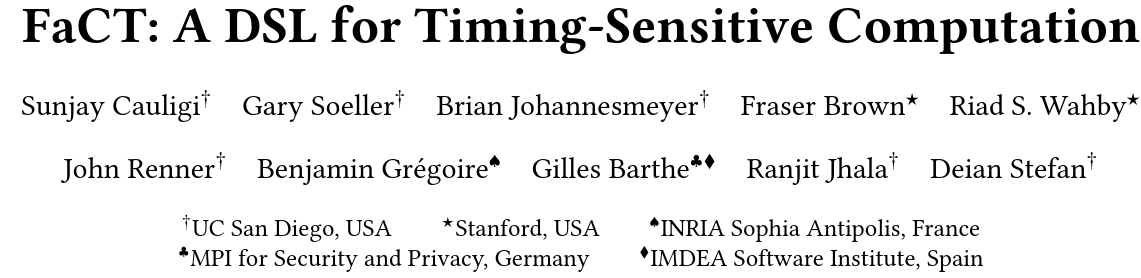
\includegraphics[width=0.8\textwidth]{../betterpl/fact-title}
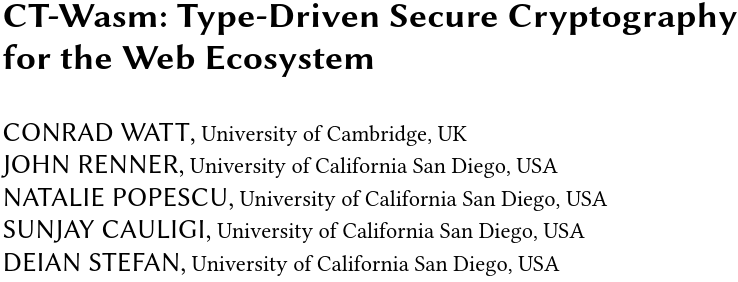
\includegraphics[width=0.8\textwidth]{../betterpl/ct-wasm-title}
\begin{itemize}
\item FaCT, PLDI 2019; CT-Wasm: POPL 2019
\end{itemize}
\end{frame}

\begin{frame}{constant-time programming languages}
    \begin{itemize}
    \item active research area, no consensus on what works best
    \vspace{.5cm}
    \item common approach: separate type for \textbf{secret} data
    \item compiler or language virtual machine disallows variable-time operations using secret data
    \item no secret-based array lookup (cache timing varies)
        \begin{itemize}
        \item e.g. array[secret\_value] $\rightarrow$ compile error (type mismatch)
        \end{itemize}
    \item no secret-based integer division (usually variable speed instruction)
    \item \ldots
    \vspace{.5cm}
    \item explicit operations for any secret-to-non-secret conversions
    \end{itemize}
\end{frame}




\section{testing for security}
\begin{frame}{on testing}
    \begin{itemize}
    \item challenges with testing for security:
    \vspace{.5cm}
    \item security bugs use ``unrealistic'' inputs --- e.g. $>8000$ character name
    \item \sout<2>{memory errors often don't crash}
        \begin{itemize}
        \item<2> bounds checking, etc. tools will fix
        \end{itemize}
    \end{itemize}
\end{frame}


\section{fuzzing, generally}

\begin{frame}{automatic testing tools}
    \begin{itemize}
        \item basic idea: generate lots of random inputs --- ``\myemph{fuzzing}''
            \begin{itemize}
            \item easy to generate weird inputs
            \end{itemize}
        \item look for memory errors
            \begin{itemize}
            \item segfaults, or
            \item use memory error detector, or
            \item add (slow) `assertions' or other checks to code
            \end{itemize}
        \vspace{.5cm}
        \item one of the most common ways to find security bugs
    \end{itemize}
\end{frame}



\subsection{``blackbox''}

\begin{frame}[fragile,label=bbFuzz]{`blackbox' fuzzing}
\lstset{
    language=C++,
    style=small,
    moredelim={**[is][\btHL<2>]{~flip~}{~end~}},
    moredelim={**[is][\btHL<3>]{~parse~}{~end~}},
}
\begin{lstlisting}
void fuzzTestImageParser(std::vector<byte> &originalImage) {
  for (int i = 0; i < NUM_TRIES; ++i) {
    std::vector<byte> testImage;
    testImage = originalImage;
    int numberOfChanges = rand() % MAX_CHANGES;
    for (int j = 0; j < numberOfChanges; ++j) {
      /* flip some random bits */
      ~flip~testImage[rand() % testImage.size()] ^= rand() % 256;~end~
    }
    int result = ~parse~TryToParseImage(testImage);~end~
    if (~parse~result == CRASH~end~) ...
  }
}
\end{lstlisting}
\end{frame}

\begin{frame}{blackbox fuzzing pros}
    \begin{itemize}
        \item works with \myemph{unmodified software}
        \begin{itemize}
            \item even with embedded assembly, etc.
        \end{itemize}
    \item works with many kinds of input
        \begin{itemize}
            \item \myemph{don't need to understand input format}
        \end{itemize}
    \item easy to \myemph{parallelize}
        \vspace{.5cm}
    \item has actually found lots of bugs
    \end{itemize}
\end{frame}

\begin{frame}{`blackbox'?}
    \begin{itemize}
    \item the program is a ``black box'' --- can't look inside
    \item we only run it, see if it works
    \item for memory errors --- works $\approx$ doesn't crash
    \end{itemize}
\end{frame}



\subsection{what can we test}
\begin{frame}{what can fuzzing find}
    \begin{itemize}
        \item easiest to find crashes
            \begin{itemize}
            \item intuition: segfault could be security problem
            \end{itemize}
        \item otherwise: how do we know if test cases are useful?
        \vspace{.5cm}
        \item need some way to know if test result is correct
        \item example: fuzz-testing of C compilers versus other C compilers
            \begin{itemize}
            \item Yang et al, ``Finding and Understanding Bugs in C compilers'', 2011
            \item 79 GCC, 209 Clang bugs
            \item about one third ``wrong generated code''
            \item but using smarter fuzzing strategy (we'll talk about it later)
            \end{itemize}
    \end{itemize}
\end{frame}



\subsection{other applications}
\begin{frame}{testing for non-memory flaws?}
    \begin{itemize}
    \item fuzzing for cross-site scripting bugs?
        \begin{itemize}
        \item run on web application
        \item assert that HTML is well-formed?
        \end{itemize}
    \item fuzzing for SQL injection?
        \begin{itemize}
        \item assert that no malformed SQL gets executed?
        \end{itemize}
    \item operating system?
        \begin{itemize}
        \item input = requests (system calls) to make to the OS
        \end{itemize}
    \vspace{.5cm}
    \item (less likely) fuzzing for permissions issues?
        \begin{itemize}
        \item assert that admin. data doesn't change?
        \end{itemize}
    \end{itemize}
\end{frame}


\subsection{some practical issues}

\begin{frame}{fuzzing challenges}
    \begin{itemize}
    \item isolation:
        \begin{itemize}
        \item need to \myemph{detect crashes}/etc. reliably
        \item want \myemph{reproducible test cases}
        \item need to distinguish \myemph{hangs} from ``machine is randomly slow''
        \end{itemize}
    \item speed:
        \begin{itemize}
            \item need to run \myemph{many millions of tests}
        \item application startup times are a problem
        \end{itemize}
    \item \textbf<2>{\myemph<2>{completeness:}}
        \begin{itemize}
            \item might have to get \textit{really} lucky to make interesting input
        \end{itemize}
    \end{itemize}
\end{frame}


\subsubsection{lots of bad tests?}

\begin{frame}{completeness problem}
    \begin{itemize}
        \item let's say we're testing an HTML parser
        \item what code is \textbf{usually} going to when we flip random bits?
            \begin{itemize} 
                \item (or remove/add random bytes)
            \end{itemize}
        \vspace{.5cm}
        \item<2> how often are we going to generate tags not in starting document?
        \item<2> how often are we going to generate new almost-valid documents?
    \end{itemize}
\end{frame}


\begin{frame}[fragile,label=HTMLchanges]{HTML with changes}
\begin{lstlisting}[
    language={},style=small,
    moredelim={**[is][\btHL<1>]{~error~}{~end~}},
]
<html><head><title>A</title></head><body>B</body></html>
<html~error~*~end~<head><title>A</title></head><body>B</body></html>
<html><~error~i~end~ead><title>~error~C~end~</title></head><body>B</body></html>
\end{lstlisting}
\end{frame}




\subsubsection{example: Yang et al}
\begin{frame}{CSmith}
    \begin{itemize}
    \item Yang et al wrote a random C program generator
        \begin{itemize}
        \item ``Finding and Understanding Ubgs in C compilers'' (PLDI 2011)
        \end{itemize}
    \vspace{.5cm}
    \item carefully avoided code with unspecified effects
        \begin{itemize}
        \item most of the work was about doing this
        \end{itemize}
    \item don't need to know what program does: comparing two compilers
        \begin{itemize}
        \item or one compiler with different settings
        \end{itemize}
    \vspace{.5cm}
    \item random selection of types, operators, etc.
    \item \ldots instead of just random bytes
    \end{itemize}
\end{frame}

\begin{frame}{CReduce}
    \begin{itemize}
    \item Regher et al (including Yang)'s follow-up work
        \begin{itemize}
        \item ``Test-Case Reduction for C Compiler Bugs'' (PLDI 2012)
        \end{itemize}
    \item take a C program that triggers bug\ldots
    \item try removing things to make it smaller
    \item needed: automated way of checking ``is bug still there''
    \vspace{.5cm}
    \item same idea applies to security bugs
        \begin{itemize}
        \item remove as much as possible and get it to still segfault
        \end{itemize}
    \end{itemize}
\end{frame}


\subsection{what makes good tests?} % FIXME: turn into exerccise?

\begin{frame}[fragile,label=testExample]{thinking about testing}
    \lstset{language=C,style=smaller}
\begin{lstlisting}
void expand(char *arg) {
    if (arg[0] == '[') {
        if (arg[2] != '-' || arg[4] != ']') {
            putchar('[');
            expand(&arg[1]);
        } else {
            for (int i = arg[1]; i <= arg[3]; ++i) {
                putchar(i);
            }
            expand(&arg[5]);
        }
    } else if (arg[0] != '\0') {
        putchar(arg[0]);
        expand(&arg[1]);
    }
}
\end{lstlisting}
\end{frame}



\section{metric: coverage}

\begin{frame}{coverage}
    \begin{itemize}
        \item ``coverage'': metric for how good tests are
        \vspace{.5cm}
        \item \myemph{\% of code reached}
        \item easy to measure
        \item correlates with bugs found
            \begin{itemize}
            \item but not the same thing as finding all bugs
            \end{itemize}
    \end{itemize}
\end{frame}

\begin{frame}{automated test generation}
    \begin{itemize}
        \item conceptual idea: look at code, go down \myemph{all paths}
    \item seems automatable?
        \begin{itemize}
        \item just need to identify conditions for each path
        \end{itemize}
    \end{itemize}
\end{frame}



\section{coverage-guided fuzzing}


\begin{frame}{a compromise: coverage-guided fuzzing}
    \begin{itemize}
    \item symbolic execution: try to maximize paths run\ldots
    \item by finding potential paths, solving to run them
    \vspace{.5cm}
    \item observation: easy to measure which paths a test case uses
        \begin{itemize}
        \item way, way, way easier than solving eqn to find a case for that path
        \end{itemize}
    \item can make random tests \myemph{biased towards finding new paths}
    \end{itemize}
\end{frame}




\subsection{examples}

\begin{frame}[fragile,label=coverageSame]{coverage-guided example}
    \lstset{language=C,style=script}
    \begin{tikzpicture}
        \node[anchor=north east] at (0, 0) {
\begin{lstlisting}
void foo(int a, int b) {
    if (a != 0) {
        // W
        b -= 2;
        a += b;
    } else {
        // X
    }
    if (b < 5) {
        // Y
        b += 4;
        if (a + b > 50) {
            // Q
            ...
        }
    } else {
        // Z
    }
}
\end{lstlisting}
};
        \tikzset{
            caseBox/.style={draw,thick,align=left,font=\small},
            variantBox/.style={draw,thick,dashed,align=left,font=\fontsize{10}{11}\selectfont},
        }
        \node[caseBox,anchor=north west] (baseA) at (1, 0) {
            initial test case A: \\ a = 0x17, b = 0x08; covers: WZ
        };
        \begin{visibleenv}<2>
            \node[anchor=north west,font=\small] at (1, -1.25) {
                generate random tests based on  A
            };
            \node[variantBox,anchor=north west] (subA) at (1, -2) {
                a = 0x37, b = 0x08; covers: WZ \\
                a = 0x15, b = 0x08; covers: WZ \\
                a = 0x17, b = 0x0c; covers: WZ \\
                a = 0x13, b = 0x08; covers: WZ \\
                a = 0x17, b = 0x08; covers: WZ \\
                \ldots \\
                a = 0x17, b = 0x00; covers: \myemph<2>{WY} 
            };
        \end{visibleenv}
        \begin{visibleenv}<3-4>
            \node[caseBox,draw=red,anchor=north west] (baseB) at (1, -1.2) {
                \myemph<3>{found } test case B: \\ a = 0x17, b = 0x00; covers: WY
            };
        \end{visibleenv}
        \begin{visibleenv}<4>
            \node[anchor=north west,font=\small] at (1, -2.5) {
                generate random tests based on A, B
            };
            \node[variantBox,anchor=north west] (subA) at (1, -3.5) {
                a = 0x37, b = 0x08; covers: WZ \\
                a = 0x04, b = 0x00; covers: WY \\
                a = 0x17, b = 0x01; covers: WZ \\
                a = 0x16, b = 0x00; covers: WY \\
                \ldots \\
                a = 0x97, b = 0x00; covers: \myemph<4>{WYQ} \\
                \ldots \\
                a = 0x00, b = 0x08; covers: \myemph<4>{XY} \\
            };
        \end{visibleenv}

    \end{tikzpicture}
\end{frame}


\begin{frame}[fragile,label=coverageExBig]{coverage-guided example}
    \lstset{language=C,style=smaller}
    \begin{tikzpicture}
        \node[anchor=north east] at (0, 0) {
\begin{lstlisting}
void foo(unsigned a,
         unsigned b,
         unsigned c) {
    if (a != 0) {
        b -= c; // W
    }
    if (b < 5) {
        if (a > c) {
            a += b; // X
        }
        b += 4; // Y
    } else {
        a += 1; // Z
    }
    assert(a + b != 7); 
}
\end{lstlisting}
};
        \tikzset{
            caseBox/.style={draw,thick,align=left,font=\small},
            variantBox/.style={draw,thick,dashed,align=left,font=\fontsize{10}{11}\selectfont},
        }
        \node[caseBox,anchor=north west] (baseA) at (1, 0) {
            initial test case A: \\ a = 0x17, b = 0x08, c = 0x00; covers: WZ
        };
        \begin{visibleenv}<2>
            \node[anchor=north west,font=\small] at (1, -1.25) {
                generate random tests based on  A
            };
            \node[variantBox,anchor=north west] (subA) at (1, -2) {
                a = 0x37, b = 0x08, c = 0x00; covers: WZ \\
                a = 0x15, b = 0x08, c = 0x02; covers: WZ \\
                a = 0x17, b = 0x0c, c = 0x00; covers: WZ \\
                a = 0x13, b = 0x08, c = 0x40; covers: WZ \\
                a = 0x17, b = 0x08, c = 0x10; covers: WZ \\
                \ldots \\
                a = 0x17, b = 0x00, c = 0x01; covers: \myemph<2>{WXY} 
            };
        \end{visibleenv}
        \begin{visibleenv}<3-4>
            \node[caseBox,draw=red,anchor=north west] (baseB) at (1, -1.2) {
                \myemph<3>{found } test case B: \\ a = 0x17, b = 0x00, c = 0x01; covers: WXY
            };
        \end{visibleenv}
        \begin{visibleenv}<4>
            \node[anchor=north west,font=\small] at (1, -2.5) {
                generate random tests based on A, B
            };
            \node[variantBox,anchor=north west] (subA) at (1, -3.5) {
                a = 0x37, b = 0x08, c = 0x00; covers: WZ \\
                a = 0x17, b = 0x00, c = 0x03; covers: WXY \\
                a = 0x17, b = 0x0c, c = 0x00; covers: WZ \\
                a = 0x37, b = 0x00, c = 0x03; covers: WXY \\
                a = 0x17, b = 0x08, c = 0x10; covers: WZ \\
                \ldots \\
                a = 0x17, b = 0x00, c = 0x81; covers: \myemph<4>{WY}
            };
        \end{visibleenv}

    \end{tikzpicture}
\end{frame}



\subsection{exercise}
\begin{frame}[fragile,label=covFuzzExercise]{exercise: coverage guidance good for?}
\begin{lstlisting}[language=C,style=smaller]
void example1(int a, int b) {
    if (a < 4 && b < 4 && a == b) {
        assert(a + b != 6);
    }
}
void example2(int a, int b) {
    assert(a != 10325);
}
void example3(int a, int b) {
    assert(a != 10325 && b != 10543);
}
\end{lstlisting}
\begin{itemize}
\item exercise: for which of these functions would coverage guided fuzzing be most/least better
than random testing for making the assertion fail?
\end{itemize}
\end{frame}


\subsection{AFL as running example}

\begin{frame}[fragile,label=afl]{american fuzzy lop}
    \begin{itemize}
        \item one example of a fuzzer that uses this strategy
            \begin{itemize}
            \item ``whitebox fuzzing''
            \end{itemize}
        \vspace{.5cm}
        \item assembler wrapper to record computed/conditional jumps:
\begin{lstlisting}
CoverageArray[Hash(JumpSource, JumpDest)]++;
\end{lstlisting}
        \item use values from coverage array to distinguish cases
        \item outputs only \myemph{unique} test cases
        \item goal: test case for every possible jump source/dest
    \end{itemize}
\end{frame}

\begin{frame}{american fuzzy lop heuristics}
    \begin{itemize}
    \item american fuzzy lop does some deterministic testing
        \begin{itemize}
        \item try flipping every bit, every 2 bits, etc. of base input
        \item overwrite bytes with 0xFF, 0x00, etc.
        \item etc.
        \end{itemize}
    \item has many strategies for producing new inputs
        \begin{itemize}
        \item bit-flipping
        \item duplicating important-looking keywords
        \item combining existing inputs
        \end{itemize}
    \end{itemize}
\end{frame}



\subsection{automatic test case simplification}
\begin{frame}[fragile,label=covMinEx]{simplifying testing cases}
\begin{lstlisting}[style=script]
int array[10];
void vulnerable(char *input) {
    char *p;
    int count = 0;
    p = input;
    if (*p == 'A') { 
        p += 1;
        while (*p == '0') {p += 1; count -= 1;}
        while (*p >= 'A' && *p < 'E') p += 1;
        while (*p == '0') {p += 1; count += 1;}
    }
    if (*p == 'B')
        array[count] += 1;
}
\end{lstlisting}
\begin{itemize}
\item example crash: {\small\texttt{A00ABDBBBDEEDDDCCCBBBDDDAAAA00000000000000000000000B}}
    \begin{itemize}
    \item might be what coverage-guided fuzzing finds
    \end{itemize}
\item would really prefer minimal example: \texttt{A00000000000B}
\end{itemize}
\end{frame}


\begin{frame}[fragile,label=covMin]{automatically simplifying test cases}
    \begin{itemize}
        \item but look for \myemph{same result and/or coverage}
        \item systematic simplifications:
            \begin{itemize}
                \item try removing every character (one-by-one)
                \item try decrementing every byte
                \item \ldots
            \end{itemize}
        \item keep simplifications that don't change result
        \item AFL uses some of this strategy to help get better `base' tests
            \begin{itemize}
            \item also has tool to do this on a found test
            \item prefers simpler `base' tests
            \end{itemize}
    \end{itemize}
\end{frame}


\subsection{AFL: test template support}

\begin{frame}{AFL: manual keywords}
    \begin{itemize}
    \item AFL supports a dictionary
        \begin{itemize}
        \item list of things to add to create test cases
        \item example: all possible HTML tags
        \end{itemize}
        \vspace{.5cm}
    \item other strategy: test-case template
    \item other strategy: test postprocessing (fix checksums, etc.)
    \end{itemize}
\end{frame}




\section{backup slides}
\begin{frame}{backup slides}
\end{frame}
\subsection{basic ownership}
\begin{frame}{rules to stop dangling pointers (1)}
    \begin{itemize}
    \item objects have an single \myemph{owner}
    \item owner is the only one allowed to modify an object
    \item owner can give away ownership
    \item simplest version: only owner can access object
    \item never have multiple references to object --- always move/copy
    \end{itemize}
\end{frame}

\begin{frame}[fragile,label=rustOwnership1]{Rust objects and ownership (1a)}
    \begin{minted}[fontsize=\fontsize{9}{10}\selectfont]{Rust}
fn mysum(vector: Vec<u32>) -> u32 {
    let mut total: u32 = 0;
    for value in &vector {
        total += value
    }
    return total
}

fn foo() {
    let vector: Vec<u32> = vec![1, 2, 3];
    let sum = mysum(vector);
    // **moves** vector into mysum()
         // philosophy: no implicit expensive copies
    
    println!("Sum is {}", sum);
    // ERROR
    println!("vector[0] is {}" , vector[0]);
}
\end{minted}
    \begin{tikzpicture}[overlay,remember picture]
        \begin{visibleenv}<2>
            \node[anchor=center,font=\small,draw=black,ultra thick,fill=white] at (current page.center){
            \begin{lstlisting}[language={},style=script]
   Compiling lecture-demo v0.1.0 (file:///home/cr4bd/spring2017/cs4630/...
error[E0382]: use of moved value: `vector`
  --> src/main.rs:16:34
   |
13 |     let sum = mysum(vector);
   |                     ------ value moved here
...
16 |     println!("vector[0] is {}" , vector[0]);
   |                                  ^^^^^^ value used here after move
\end{lstlisting}
        };
        \end{visibleenv}
    \end{tikzpicture}
\end{frame}

\begin{frame}[fragile,label=rustOwnership2]{Rust objects and ownership (2)}
    \begin{minted}[fontsize=\fontsize{9}{10}\selectfont]{Rust}
fn mysum(vector: Vec<u32>) -> u32 {
    let mut total: u32 = 0
    for value in &vector {
        total += value
    }
    return total
}

fn foo() {
    let vector: Vec<u32> = vec![1, 2, 3];
    let sum = mysum(vector.clone());
    // give away a copy of vector instead
        // mysum will dispose, since it owns it
    
    println!("Sum is {}", sum);
    println!("vector[0] is {}" , newVector[0]);
}
\end{minted}
    \begin{tikzpicture}[overlay,remember picture]
        \begin{visibleenv}<2>
            \node[anchor=center,font=\small,draw=black,ultra thick,fill=white,align=center] at (current page.center){
            mysum borrows a copy
        };
        \end{visibleenv}
    \end{tikzpicture}
\end{frame}

\begin{frame}{moving?}
    \begin{itemize}
    \item moving a Vec --- really copying a pointer to an array and its size
    \item cloning a Vec --- making a copy of the array itself, too
    \vspace{.5cm}
    \item Rust defaults to moving non-trivial types
    \item some trivial types (u32, etc.) are copied by default
    \end{itemize}
\end{frame}

\begin{frame}[fragile,label=rustOwnership3]{Rust objects and ownership (3)}
    \begin{minted}[fontsize=\fontsize{9}{10}\selectfont]{Rust}
fn mysum(vector: Vec<u32>) -> (u32, Vec<u32>) {
    let mut total: u32 = 0
    for value in &vector {
        total += value
    }
    return (total, vector)
}

fn foo() {
    let vector: Vec<u32> = vec![1, 2, 3];
    let (sum, newVector) = mysum(vector);
    // give away vector, get it back
    
    println!("Sum is {}", sum);
    println!("vector[0] is {}" , newVector[0]);
}
\end{minted}
    \begin{tikzpicture}[overlay,remember picture]
        \begin{visibleenv}<2>
        \node[anchor=center,font=\small,draw=black,ultra thick,align=center,fill=white] 
            at (current page.center) {
        mysum ``borrows'' vector, then gives it back \\
        uses pointers
        };
        \end{visibleenv}
    \end{tikzpicture}
\end{frame}

\begin{frame}{ownership rules}
    \begin{itemize}
    \item exactly one owner at a time
    \item giving away ownership means you \myemph{can't use object}
        \begin{itemize}
        \item<2> common idiom --- temporarily give away object
        \end{itemize}
    \item either give object new owner or deallocate
    \end{itemize}
\end{frame}



\end{document}
